\documentclass{article}
\usepackage[utf8]{inputenc}
\usepackage{enumerate}
\usepackage{amsmath}
\usepackage{amssymb}
\usepackage{amsfonts}
\usepackage{amstext}
\usepackage{amsthm}
\usepackage{mathtools}
\usepackage{tikz}
\usepackage{amsmath}
\usepackage{cancel}
\DeclarePairedDelimiter{\ceil}{\lceil}{\rceil}
\title{Calculus III Review Sheet 1 Practice}
\author{Eddie Ozuna and Tyler Franklin}

\begin{document}
\maketitle
\section{Dot Products}
\begin{enumerate}[a.]
	\item \textbf{What is the geometric significance of the dot product? }\\
	\\
Two vectors are orthogonal(Perpendicular) if and only if the result of the dot product is equal to zero.\\\\
$\vec{u} = <u_{1},u_{2},u_{3}>\hspace{.4cm}\vec{v} = <v_{1},v_{2},v_{3}>$\\
\\
Reminder in how to perform the dot product:\\
\\
$\vec{u} \cdot \vec{v} = (u_{1} \cdot v_{1}) + (u_{2} \cdot v_{2}) + (u_{3} \cdot v_{3}) $\\
\\
Another Approach in how to perform the dot product:\\
\\
$\vec{u} \cdot \vec{v} =  \mid\vec{u}\mid\mid\vec{v}\mid\cos(\theta)$\\
\\
$\mid\vec{u}\mid = \sqrt{u_{1}\hspace{.001cm}^{2}+u_{2}\hspace{.001cm}^{2}+u_{3}\hspace{.001cm}^{2}}$\\
\\
$\mid\vec{v}\mid = \sqrt{v_{1}\hspace{.001cm}^{2}+v_{2}\hspace{.001cm}^{2}+v_{3}\hspace{.001cm}^{2}}$\\
\\
$\theta$ = The angle between the two vectors $\vec{u}$ and $\vec{v}$
\end{enumerate}
\begin{enumerate}[b.]
	\item \textbf{Why does the dot product have such geometric significance? Can you prove it? Hint: Remember the Pythagorean Theorem and its degeneration into the Law of Cosines. Can
you draw a picture to describe the scenario? }\\
	\\
	Given the definition above, where $\theta$ is the angle between $\vec{u}$ and $\vec{v}$, we can be certain that a result of $0$ means $\cos(\theta)=0$ which in turn means $\theta=\frac{\pi}{2}$ or $\theta=\frac{3\pi}{2}$ i.e. either a 90$^{\circ}$ or 270$^{\circ}$ perpendicular angle.\\
	
	Derivation: Law of Cosine\\
	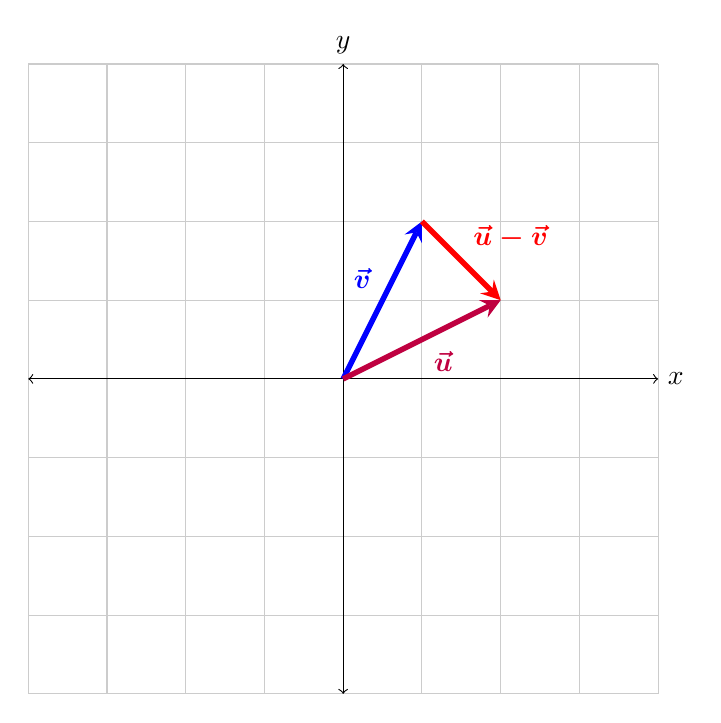
\begin{tikzpicture}
  \draw[thin,gray!40] (-4,-4) grid (4,4);
  \draw[<->] (-4,0)--(4,0) node[right]{$x$};
  \draw[<->] (0,-4)--(0,4) node[above]{$y$};
  \draw[line width=2pt,blue,-stealth](0,0)--(1,2) coordinate (VecV) node[midway,auto]{$\boldsymbol{\vec{v}}$};
  \draw[line width=2pt,purple,-stealth](0,0)--(2,1) coordinate (VecU) node[midway,auto,swap]{$\boldsymbol{\vec{u}}$};
  \draw[line width=2pt,red,-stealth](1,2)--(2,1) node[midway,auto]{$\boldsymbol{\vec{u}-\vec{v}}$};
  
\end{tikzpicture}\\
\\
	$\mid\vec{u}-\vec{v}\mid^{2} = \mid\vec{u}\mid^{2} + \mid\vec{v}\mid^{2}-\hspace{.1cm}2\mid\vec{u}\mid\cdot\mid\vec{v}\mid\cos(\theta)$\\
\\
$\cancel{\mid\vec{u}\mid^{2}}-\hspace{.1cm}2\vec{v}\cdot\vec{u}\hspace{.1cm}+\cancel{\mid\vec{v}\mid^{2}}=\cancel{\mid\vec{u}\mid^{2}} + \cancel{\mid\vec{v}\mid^{2}}-2\mid\vec{u}\mid\cdot\mid\vec{v}\mid\cos(\theta)$\\
\\
$\cancel{-2}\vec{v}\cdot\vec{u} = \cancel{-2}\mid\vec{u}\mid\cdot\mid\vec{v}\mid\cos(\theta)$\\
\\
$\vec{v}\cdot\vec{u} = \mid\vec{u}\mid\cdot\mid\vec{v}\mid\cos(\theta)$\\
\end{enumerate}
\section{.}
\begin{enumerate}[a.]
\item \textbf{What is the geometric significance of the cross product of two vectors?}\\
\\
It will always yield a new vector that is orthogonal(perpendicular) to the two vectors you took the cross product.\\
\\

$\hspace{1cm}\hat{i}\hspace{.4cm}\hat{j}\hspace{.3cm}\hat{k}\hspace{2cm}\hat{i}\hspace{.4cm}\hat{j}\hspace{.3cm}\hat{k}\\\vec{u} = <u_{1},u_{2},u_{3}>\hspace{.4cm}\vec{v} = <v_{1},v_{2},v_{3}>$\\
\\
Reminder in how to perform the cross product:\\
\\
$\vec{u}\times\vec{v}=\begin{vmatrix}
\hat{i}&\hat{j}&\hat{k}\\
u_{1}&u_{2}&u_{3}\\
v_{1}&v_{2}&v_{3}\\
\end{vmatrix}=\hat{i}
\begin{vmatrix}
u_{2}&u_{3}\\
v_{2}&v_{3}\\
\end{vmatrix}-\hat{j}\begin{vmatrix}
u_{1}&u_{3}\\
v_{1}&v_{3}\\
\end{vmatrix}+\hat{k}\begin{vmatrix}
u_{1}&u_{2}\\
v_{1}&v_{2}\\
\end{vmatrix}\\
=\hat{i}(u_{2}v_{3}-u_{3}v_{2})-\hat{j}(u_{1}v_{3}-u_{3}v_{1})+\hat{k}(u_{1}v_{2}-u_{2}v_{1})$\\
\\
Another Approach in how to perform the cross product:\\
\\
$\vec{u} \times \vec{v} =  \mid\vec{u}\mid\mid\vec{v}\mid\sin(\theta)$\\
\\
$\mid\vec{u}\mid = \sqrt{u_{1}\hspace{.001cm}^{2}+u_{2}\hspace{.001cm}^{2}+u_{3}\hspace{.001cm}^{2}}$\\
\\
$\mid\vec{v}\mid = \sqrt{v_{1}\hspace{.001cm}^{2}+v_{2}\hspace{.001cm}^{2}+v_{3}\hspace{.001cm}^{2}}$\\
\\
$\theta$ = The angle between the two vectors $\vec{u}$ and $\vec{v}$
\end{enumerate}
\begin{enumerate}[b.]
\item \textbf{Why does the cross product have such geometric significance?}\\
\\
\end{enumerate}
\section{.}
\begin{enumerate}[a.]
\item \textbf{Prove that the cross product $\vec{u} \times \vec{v}$ of two vectors $\vec{u}$ and $\vec{v}$ is actually orthogonal(perpendicular) to each of $\vec{u}$ and $\vec{v}$ simultaneously.}\\
\\

$\hspace{1cm}\hat{i}\hspace{.4cm}\hat{j}\hspace{.3cm}\hat{k}\hspace{2cm}\hat{i}\hspace{.4cm}\hat{j}\hspace{.3cm}\hat{k}\\\vec{u} = <u_{1},u_{2},u_{3}>\hspace{.4cm}\vec{v} = <v_{1},v_{2},v_{3}>$\\
\\
Step 1. Take the cross product of $\vec{u}$ and $\vec{v}$\\
\\
$\vec{u}\times\vec{v}=\begin{vmatrix}
\hat{i}&\hat{j}&\hat{k}\\
u_{1}&u_{2}&u_{3}\\
v_{1}&v_{2}&v_{3}\\
\end{vmatrix}=\hat{i}
\begin{vmatrix}
u_{2}&u_{3}\\
v_{2}&v_{3}\\
\end{vmatrix}-\hat{j}\begin{vmatrix}
u_{1}&u_{3}\\
v_{1}&v_{3}\\
\end{vmatrix}+\hat{k}\begin{vmatrix}
u_{1}&u_{2}\\
v_{1}&v_{2}\\
\end{vmatrix}\\
=\hat{i}(u_{2}v_{3}-u_{3}v_{2})-\hat{j}(u_{1}v_{3}-u_{3}v_{1})+\hat{k}(u_{1}v_{2}-u_{2}v_{1})$\\
\\
Let define $\vec{w}$ to be equal to the result of the cross product of $\vec{u}$ and $\vec{v}$\\
$\vec{w} = \hat{i}(u_{2}v_{3}-u_{3}v_{2})-\hat{j}(u_{1}v_{3}-u_{3}v_{1})+\hat{k}(u_{1}v_{2}-u_{2}v_{1})$\\
\\
Step 2. From our previous knowledge we know that if the result of the dot product is zero the vectors are orthogonal(perpendicular). With that being said let perform the dot products of vector $\vec{u}$ with $\vec{w}$ and $\vec{v}$ with $\vec{w}$.\\
\\
$\vec{w} = <(u_{2}v_{3}-u_{3}v_{2}),-(u_{1}v_{3}-u_{3}v_{1}),(u_{1}v_{2}-u_{2}v_{1})>$\\
\\
$\vec{u}\cdot\vec{w}=u_{1}(u_{2}v_{3}-u_{3}v_{2})-u_{2}(u_{1}v_{3}-u_{3}v_{1})+u_{3}(u_{1}v_{2}-u_{2}v_{1})\\=u_{1}u_{2}v_{3}-u_{1}v_{2}u_{3}-u_{1}u_{2}v_{3}+v_{1}u_{2}u_{3}+u_{1}u_{3}v_{2}-v_{1}u_{2}u_{3}=0$\\
\\ 
$\vec{v}\cdot\vec{w}=v_{1}(u_{2}v_{3}-u_{3}v_{2})-v_{2}(u_{1}v_{3}-u_{3}v_{1})+v_{3}(u_{1}v_{2}-u_{2}v_{1})\\=v_{1}u_{2}v_{3}-v_{1}v_{2}u_{3}-u_{1}v_{2}v_{3}+v_{1}v_{2}u_{3}+u_{1}v_{2}v_{3}-v_{1}u_{2}v_{3}=0$\\
\\
Proven Both yield a result of zero which state they are orthogonal(perpendicular) simultaneously.
\end{enumerate}
\begin{enumerate}[b.]
\item\textbf{Find a vector that is orthogonal(perpendicular) to each of the vectors $e_{1}:= \left(\!
    \begin{array}{c}
      1 \\
      0 \\
      0
    \end{array}
  \!\right)$ and $e_{2}:=\left(\!
    \begin{array}{c}
      0 \\
      1 \\
      0
    \end{array}
  \!\right)$}
  \\
  \\
  From previous knowledge we know that taking the cross product of two vectors yield us a new vector that is orthogonal(perpendicular) to does two vectors. With that being said let perform the cross products of $e_{1}$ with $e_{2}$.
\\\\
$e_{1}=<1,0,0>\hspace{.4cm}e_{2}=<0,1,0>$\\
\\
$e_{1} \times e_{2}=\begin{vmatrix}
\hat{i}&\hat{j}&\hat{k}\\
1&0&0\\
0&1&0\\
\end{vmatrix}=\hat{i}\begin{vmatrix}
0&0\\
1&0\\
\end{vmatrix}-\hat{j}\begin{vmatrix}
1&0\\
0&0\\
\end{vmatrix}+\hat{k}\begin{vmatrix}
1&0\\
0&1\\
\end{vmatrix}=0\hat{i}-0\hat{j}+1\hat{k}$\\
\\
Let $e_{3}$ equal the result of the cross  products of $e_{1}$ with $e_{2}$.\\
\\
$e_{3}=<0,0,1>$
\end{enumerate}
\begin{enumerate}[c.]
\item\textbf{Prove that your vector is actually perpendicular to each of $e_{1}$ and $e_{2}$ simultaneously}\\
\\
From our previous knowledge we know that if the result of the dot product is zero the vectors are orthogonal(perpendicular). With that being said let perform the dot products of vector $e_{1}$ with $e_{3}$ and $e_{2}$ with $e_{3}$.\\
\\
$e_{1}=<1,0,0>\hspace{.4cm}e_{2}=<0,1,0>\hspace{.4cm}e_{3}=<0,0,1>$\\
\\
$e_{1} \cdot e_{3}=(1 \cdot 0) + (0 \cdot 0 ) + (0 \cdot 1) = 0$\\
\\
$e_{2} \cdot e_{3}=(0 \cdot 0) + (1 \cdot 0 ) + (0 \cdot 1) = 0$\\
\\
Proven Both yield a result of zero which state they are orthogonal(perpendicular)
\end{enumerate}
\section{}
\begin{enumerate}[a.]
\item\textbf{The volume of the parallelopiped (three-dimensional analogue of a parallelo-
gram) spanned by three vectors $\vec{u}$, $\vec{v}$ and $\vec{w}$ is given by:}\\
\\
$(\vec{u}\times\vec{v})\cdot\vec{w}:=<\vec{u}\times\vec{v},\vec{w}>$\\
\\ This just mean take the cross product of $\vec{u}$ with $\vec{v}$ and then take the dot product of the result with $\vec{w}$. Both side mean the same thing just different notation for the dot product!\\
\\
\textbf{This is known as the triple product of $\vec{u}$, $\vec{v}$ and $\vec{w}$. Interestingly enough, this is a way of defining the determinant of a matrix. Given a matrix:}\\
\\
$M:=\begin{vmatrix}
u_{1}&v_{1}&w_{1}\\
u_{2}&v_{2}&w_{2}\\
u_{3}&v_{3}&w_{3}\\
\end{vmatrix}$\\
\\
\textbf{where we notice that the columns of the matrix are precisely the vectors $\vec{u}$, $\vec{v}$ and $\vec{w}$. we can actually define the determinant of the matrix M via:}\\
\\
$det(M ) := <\vec{u}\times\vec{v},\vec{w}>$\\
\\
\textbf{Prove that these two definitions yield the same thing! The determinant of a
matrix is said to encode the amount that the unit parallelopiped is scaled upon
applying the linear transformation of space represented by the matrix.}\\
\\
To prove this we just need to take the determinant of M which is the left side of the equation and them evaluate the right side of the question which just mean take the cross product of $\vec{u}$ with $\vec{v}$ and then take the dot product of the result with $\vec{w}$.\\
\\
Left side of the equation:\\
\\
$det(M ) := \begin{vmatrix}
u_{1}&v_{1}&w_{1}\\
u_{2}&v_{2}&w_{2}\\
u_{3}&v_{3}&w_{3}\\
\end{vmatrix}=u_{1}\begin{vmatrix}
v_{2}&w_{2}\\
v_{3}&w_{3}\\
\end{vmatrix}-v_{1}\begin{vmatrix}
u_{2}&w_{2}\\
u_{3}&w_{3}\\
\end{vmatrix}+w_{1}\begin{vmatrix}
u_{2}&v_{2}\\
u_{3}&v_{3}\\
\end{vmatrix}\\\\:=u_{1}(v_{2}w_{3} - w_{2}v_{3}) - v_{1}(u_{2}w_{3}-w_{2}u_{3})+w_{1}(u_{2}v_{3}-v_{2}u_{3})\\:=u_{1}v_{2}w_{3} - u_{1}w_{2}v_{3}-v_{1}u_{2}w_{3}+v_{1}w_{2}u_{3}+w_{1}u_{2}v_{3}-w_{1}v_{2}u_{3}$\\
\\
\\
Right side of the equation:\\
\\
$<\vec{u}\times\vec{v},\vec{w}>$\\
\\
$\vec{u}\times\vec{v}=\begin{vmatrix}
\hat{i}&\hat{j}&\hat{k}\\
u_{1}&u_{2}&u_{3}\\
v_{1}&v_{2}&v_{3}\\
\end{vmatrix}=\hat{i}
\begin{vmatrix}
u_{2}&u_{3}\\
v_{2}&v_{3}\\
\end{vmatrix}-\hat{j}\begin{vmatrix}
u_{1}&u_{3}\\
v_{1}&v_{3}\\
\end{vmatrix}+\hat{k}\begin{vmatrix}
u_{1}&u_{2}\\
v_{1}&v_{2}\\
\end{vmatrix}\\
=\hat{i}(u_{2}v_{3}-u_{3}v_{2})-\hat{j}(u_{1}v_{3}-u_{3}v_{1})+\hat{k}(u_{1}v_{2}-u_{2}v_{1})$\\
\\
$<\vec{u}\times\vec{v},\vec{w}> := w_{1}(u_{2}v_{3}-u_{3}v_{2})-w_{2}(u_{1}v_{3}-u_{3}v_{1})+w_{3}(u_{1}v_{2}-u_{2}v_{1})\\:=w_{1}u_{2}v_{3}-w_{1}u_{3}v_{2}-w_{2}u_{1}v_{3}+w_{2}u_{3}v_{1}+w_{3}u_{1}v_{2}-w_{3}u_{2}v_{1}$\\
\\
You can clearly see that they are equal to each other proven!
\end{enumerate}
\begin{enumerate}[b.]
\item\textbf{Draw the result of applying this linear transformation to the unit parallelopiped spanned by the basis vectors $\vec{e_{1}}$ , $\vec{e_{2}}$ , and $\vec{e_{3}}$. The volume of the unit parallelop-iped is, of course, 1·1·1 = 1.}\\
\\
\end{enumerate}
\begin{enumerate}[c.]
\item\textbf{What is the volume of the new parallelopiped after
the linear transformation described by the matrix? Compute the determinant
of this matrix, and also the quantity and verify that they are equal, verifying that, at least in this case, the determi-nant of the matrix describing the linear transformation does in fact encode the change in volume of the unit parallelopiped under this transformation of space!}\\
\\
Just evaluate each one and check if the results are equal.\\
1.)
  $M:=\left(\!
    \begin{array}{c}
      1 \hspace{.5cm} 2 \hspace{.5cm} 3 \\
      4 \hspace{.5cm} 5 \hspace{.5cm} 6 \\
      7 \hspace{.5cm} 8 \hspace{.5cm} 8 \\
    \end{array}
  \!\right)$\\
  \\  
  \\
  \\
  $det(M ) := \begin{vmatrix}
1&2&3\\
4&5&6\\
7&8&8\\
\end{vmatrix}:=1\begin{vmatrix}
5&6\\
8&8\\
\end{vmatrix}-2\begin{vmatrix}
4&6\\
7&8\\
\end{vmatrix}+3\begin{vmatrix}
4&5\\
7&8\\
\end{vmatrix}\\:=1(5\cdot8-6\cdot8)-2(4\cdot8-6\cdot7)+3(4\cdot8-5\cdot7)\\:=-8+20-9:=3$\\
\\
 2.)
 $<\vec{u}:=\left(\!
    \begin{array}{c}
      1 \\
      4 \\
      7
    \end{array}
  \!\right)\times\vec{v}:=\left(\!
    \begin{array}{c}
      2 \\
      5 \\
      8
    \end{array}
  \!\right),\vec{w}:=\left(\!
    \begin{array}{c}
      3 \\
      6 \\
      8
    \end{array}
  \!\right)>$\\ 
$\vec{u}\times\vec{v}=\begin{vmatrix}
\hat{i}&\hat{j}&\hat{k}\\
1&4&7\\
2&5&8\\
\end{vmatrix}=\hat{i}\begin{vmatrix}
4&7\\
5&8\\
\end{vmatrix}-\hat{j}\begin{vmatrix}
1&7\\
2&8\\
\end{vmatrix}+\hat{k}\begin{vmatrix}
1&4\\
2&5\\
\end{vmatrix}\\ = \hat{i}(4 \cdot 8-7 \cdot5)-\hat{j}(1\cdot8-7\cdot2)+\hat{j}(1\cdot5-4\cdot2)\\=-3\hat{i}+6\hat{j}-3\hat{k}$\\
\\
$<\vec{u}\times\vec{v},\vec{w}>=(-3\cdot3)+(6\cdot6)+(-3\cdot8)=3 $\\
\end{enumerate}
\section{}
\begin{enumerate}[a.]
\item\textbf{Find a line passing through the point $\left(\!
    \begin{array}{c}
      1 \\
      2 \\
      3
    \end{array}
  \!\right)$ normal to the plane passing through $\left(\!
    \begin{array}{c}
      2 \\
      3 \\
      4
    \end{array}
  \!\right)$,$\left(\!
    \begin{array}{c}
      5 \\
      6 \\
      7
    \end{array}
  \!\right)$, and $\left(\!
    \begin{array}{c}
      8 \\
      9 \\
      9
    \end{array}
  \!\right)$ }\\
\\
Step 1. Find the equation of the plane passing through $\left(\!
    \begin{array}{c}
      2 \\
      3 \\
      4
    \end{array}
  \!\right)$,$\left(\!
    \begin{array}{c}
      5 \\
      6 \\
      7
    \end{array}
  \!\right)$, and $\left(\!
    \begin{array}{c}
      8 \\
      9 \\
      9
    \end{array}
  \!\right)$\\
  \\
  Let $\vec{p}=<2,3,4>, \vec{q}=<5,6,7>,$ and $\vec{k}=<8,9,9>$\\
  \\
  Let $\vec{pq} = <5-2,6-3,7-4>=<3,3,3>$\\
  \\
  Let $\vec{pk} = <8-5,9-6,9-7>=<3,3,2>$\\
  \\
  Take the cross product of vectors $\vec{pq}$ with $\vec{pk}$\\
  \\
  $\vec{pq}\times\vec{pk}=\begin{vmatrix}
\hat{i}&\hat{j}&\hat{k}\\
3&3&3\\
3&3&2\\
\end{vmatrix}=\hat{i}\begin{vmatrix}
3&3\\
3&2\\
\end{vmatrix}-\hat{j}\begin{vmatrix}
3&3\\
3&2\\
\end{vmatrix}+\hat{k}\begin{vmatrix}
3&3\\
3&3\\
\end{vmatrix}\\
=\hat{i}(3 \cdot 2-3 \cdot3)-\hat{j}(3\cdot2-3\cdot3)+\hat{j}(3\cdot3-3\cdot3)
\\=-3\hat{i}+3\hat{j}+0\hat{k}$\\
\\
General form of a equation of a plane a(x-$x_{0}$)+b(y-$y_{0}$)+c(z-$z_{0}$)=0\\
\\
$\vec{pq}\times\vec{pk}=<-3,3,0>$\\
\\
a = -3 , b = 3 , c = 0\\
\\
plane = -3(x-2)+3(y-3)+0(z-4)=0
\\
\\
normal vector $\vec{n}=<-3,3,0>$ \\
\\
\\
Step 2. Parameterized using the normal vector of the equation of the plane to get the equation of the lines using the point $<1,2,3>$\\
\\
x(t)=1-3t\\
y(t)=2+3t\\
z(t)=3+0t\\
  
\end{enumerate}
\end{document}

